%Notes by Harsh Mistry 
%Econ 301
%Based on Template From  https://www.cs.cmu.edu/~ggordon/10725-F12/template.tex

\documentclass[twoside]{article}
\setlength{\oddsidemargin}{0.25 in}
\setlength{\evensidemargin}{-0.25 in}
\setlength{\topmargin}{-0.6 in}
\setlength{\textwidth}{6.5 in}
\setlength{\textheight}{8.5 in}
\setlength{\headsep}{0.75 in}
\setlength{\parindent}{0 in}
\setlength{\parskip}{0.1 in}
\usepackage{amsmath,amsfonts,graphicx, color}
\newcounter{lecnum}
\renewcommand{\thepage}{\thelecnum-\arabic{page}}
\renewcommand{\thesection}{\thelecnum.\arabic{section}}
\renewcommand{\theequation}{\thelecnum.\arabic{equation}}
\renewcommand{\thefigure}{\thelecnum.\arabic{figure}}
\renewcommand{\thetable}{\thelecnum.\arabic{table}}
\newcommand{\lecture}[4]{
   \pagestyle{myheadings}
   \thispagestyle{plain}
   \newpage
   \setcounter{lecnum}{#1}
   \setcounter{page}{1}
   
   
%Info Box 
   \begin{center}
   \framebox{
      \vbox{\vspace{2mm}
    \hbox to 6.28in { {\bf Econ 301 - Microeconomic Theory 2
	\hfill Winter 2018} }
       \vspace{4mm}
       \hbox to 6.28in { {\Large \hfill Lecture #1: #2  \hfill} }
       \vspace{2mm}
       \hbox to 6.28in { {\it Lecturer: #3 \hfill Notes By: #4} }
      \vspace{2mm}}
   }
   \end{center}
   
   \markboth{Lecture #1: #2}{Lecture #1: #2}



 
}

\renewcommand{\cite}[1]{[#1]}
\def\beginrefs{\begin{list}%
        {[\arabic{equation}]}{\usecounter{equation}
         \setlength{\leftmargin}{2.0truecm}\setlength{\labelsep}{0.4truecm}%
         \setlength{\labelwidth}{1.6truecm}}}
\def\endrefs{\end{list}}
\def\bibentry#1{\item[\hbox{[#1]}]}

\newcommand{\fig}[3]{
			\vspace{#2}
			\begin{center}
			Figure \thelecnum.#1:~#3
			\end{center}
	}
	
	\graphicspath{ {images/} }

\newtheorem{theorem}{Theorem}[lecnum]
\newtheorem{lemma}[theorem]{Lemma}
\newtheorem{ex}[theorem]{Example}
\newtheorem{proposition}[theorem]{Proposition}
\newtheorem{claim}[theorem]{Claim}
\newtheorem{corollary}[theorem]{Corollary}
\newtheorem{definition}[theorem]{Definition}
\newenvironment{proof}{{\bf Proof:}}{\hfill\rule{2mm}{2mm}}
\newcommand\E{\mathbb{E}}


%Start of Document 
\begin{document}

\lecture{19}{March 21, 2018}{Jean Guillaume Forand}{Harsh Mistry}


\section{Externalities Continued}
\textcolor{blue}{
\textbf{Note :} This lecture builds upon the example in Lecture 17}\\

\textbf{Second solution for externalities : Government intervention through permit system}

\begin{definition} \underline{Permit System} is a framework where in order to consume one unit of a good, consumers need to pay cost \(c > 0\) for a permit
\end{definition}

\begin{itemize}
\item Suppose government expropriates all endowments of good 2 in the economy. Basically, permits must be bought for good 2.
\item We need to specify what the government does with the revenue it collects from permit sales. We can assume that the revenue is returned to consumers and shared equally. 
\item There is a competitive market for good 1 that determines its equilibria price. 
\item Given a permit price \(c\), a \underline{competitive equilibrium} is price \(p^*\), allocations \(x^{A*}\), \(x^{B*}\), and per-capita tax return \(T^*\) that satisfy
\begin{enumerate}
\item Given \(p_1^*\) and \(c\), \(x_A^*\) is a solution to 
\[\max_{x_1^A, x_2^A \geq 0} x_1^{A \frac{1}{2}} x_2^{A \frac{1}{2}} \hspace{0.2cm} \text{ s.t } \hspace{0.2cm} p_1^* x_1^A + c x_2^A \leq 2p_1^* + T^*\]
\(x^{B*}\) is a solution to
\[\max_{x_1^B, x_2^B \geq 0} x_1^{B \frac{1}{2}} [2-x_2^{A*}]^{\frac{1}{2}} \hspace{0.2cm}  \text{ s.t } \hspace{0.2cm} p_1^* x_1^B + c x_2^B \leq 2p_1^* + T^*\]
\item \(x_1^{A*} + x_1^{B*} = 2\) (MC1)
\begin{itemize}
\item There is no market clearing condition for good 2, since there is no competitive market for good 2.
\end{itemize}
\item Governments budget it balanced : 
\[2T^* = c \cdot [x_2^{A*} + x_2^{B*}]\]
\end{enumerate}
\item Demand functions are : 
\[(x_1^A(p_1, c, T), x_2^A (p_1, c, T)) = \left( \frac{2p_1 + T}{2p_1}, \frac{2p_1 + T}{2c}
\right)\]
\[(x_1^B(p_1, c, T), x_2^B (p_1, c, T)) = \left( \frac{p_1 + T}{p_1} , 0 \right)\]
\item Evaluate (MC1) 
\[\begin{aligned}
\frac{2p_1^* + T^*}{2p_1} + \frac{p_1 + T^*}{p_1} & = 3\\
\implies T^* & = \frac{2}{3} p_1^*
\end{aligned}\]
\item Evaluate balanced budget condition (BB).
\[\begin{aligned}
2T^* = c \cdot \left[\frac{2p_1^* + T^*}{2c} \right] \implies T^* = \frac{2}{3} p_1^*
\end{aligned}\]
\item This displays the (MC1) holds \(\iff\) (BB) holds
\item Normalize \(p_1^* = 1\), then \(T^* = \frac{2}{3}\)
\item Given \(c\), price \(p_1^* =1\), tax return \(T^* = \frac{2}{3}\), and allocations \(x^{A*} = \left(\frac{4}{3}, \frac{4}{3c}\right)\) and \(x^{B*} = \left(\frac{5}{3}, 0\right)\) form a competitive equilibrium
\item Are competitive equilibrium allocations with government intervention Pareto-efficient?
\[\begin{aligned}
\frac{\frac{d}{dx_1^A} u^A(x_1^{A*}, x_2^{A*})}{\frac{d}{dx_2^A} u^A(x_1^{A*}, x_2^{A*})} = \frac{x_2^{A*}}{x_1^{A*}} = \frac{1}{c} 
\end{aligned}\]
\[
\frac{\frac{d}{dx_1^B} u^B(x_1^{B*}, 2 - x_2^{A*})}{\frac{d}{dx_2^B} u^B(x_1^{B*}, 2 - x_2^{A*})} = \frac{2-x_2^{A*}}{x_1^{B*}} = \frac{6c-4}{5c}\]
\[MRS^A \geq MRS^B \iff c \leq \frac{3}{2}\]
\begin{center}
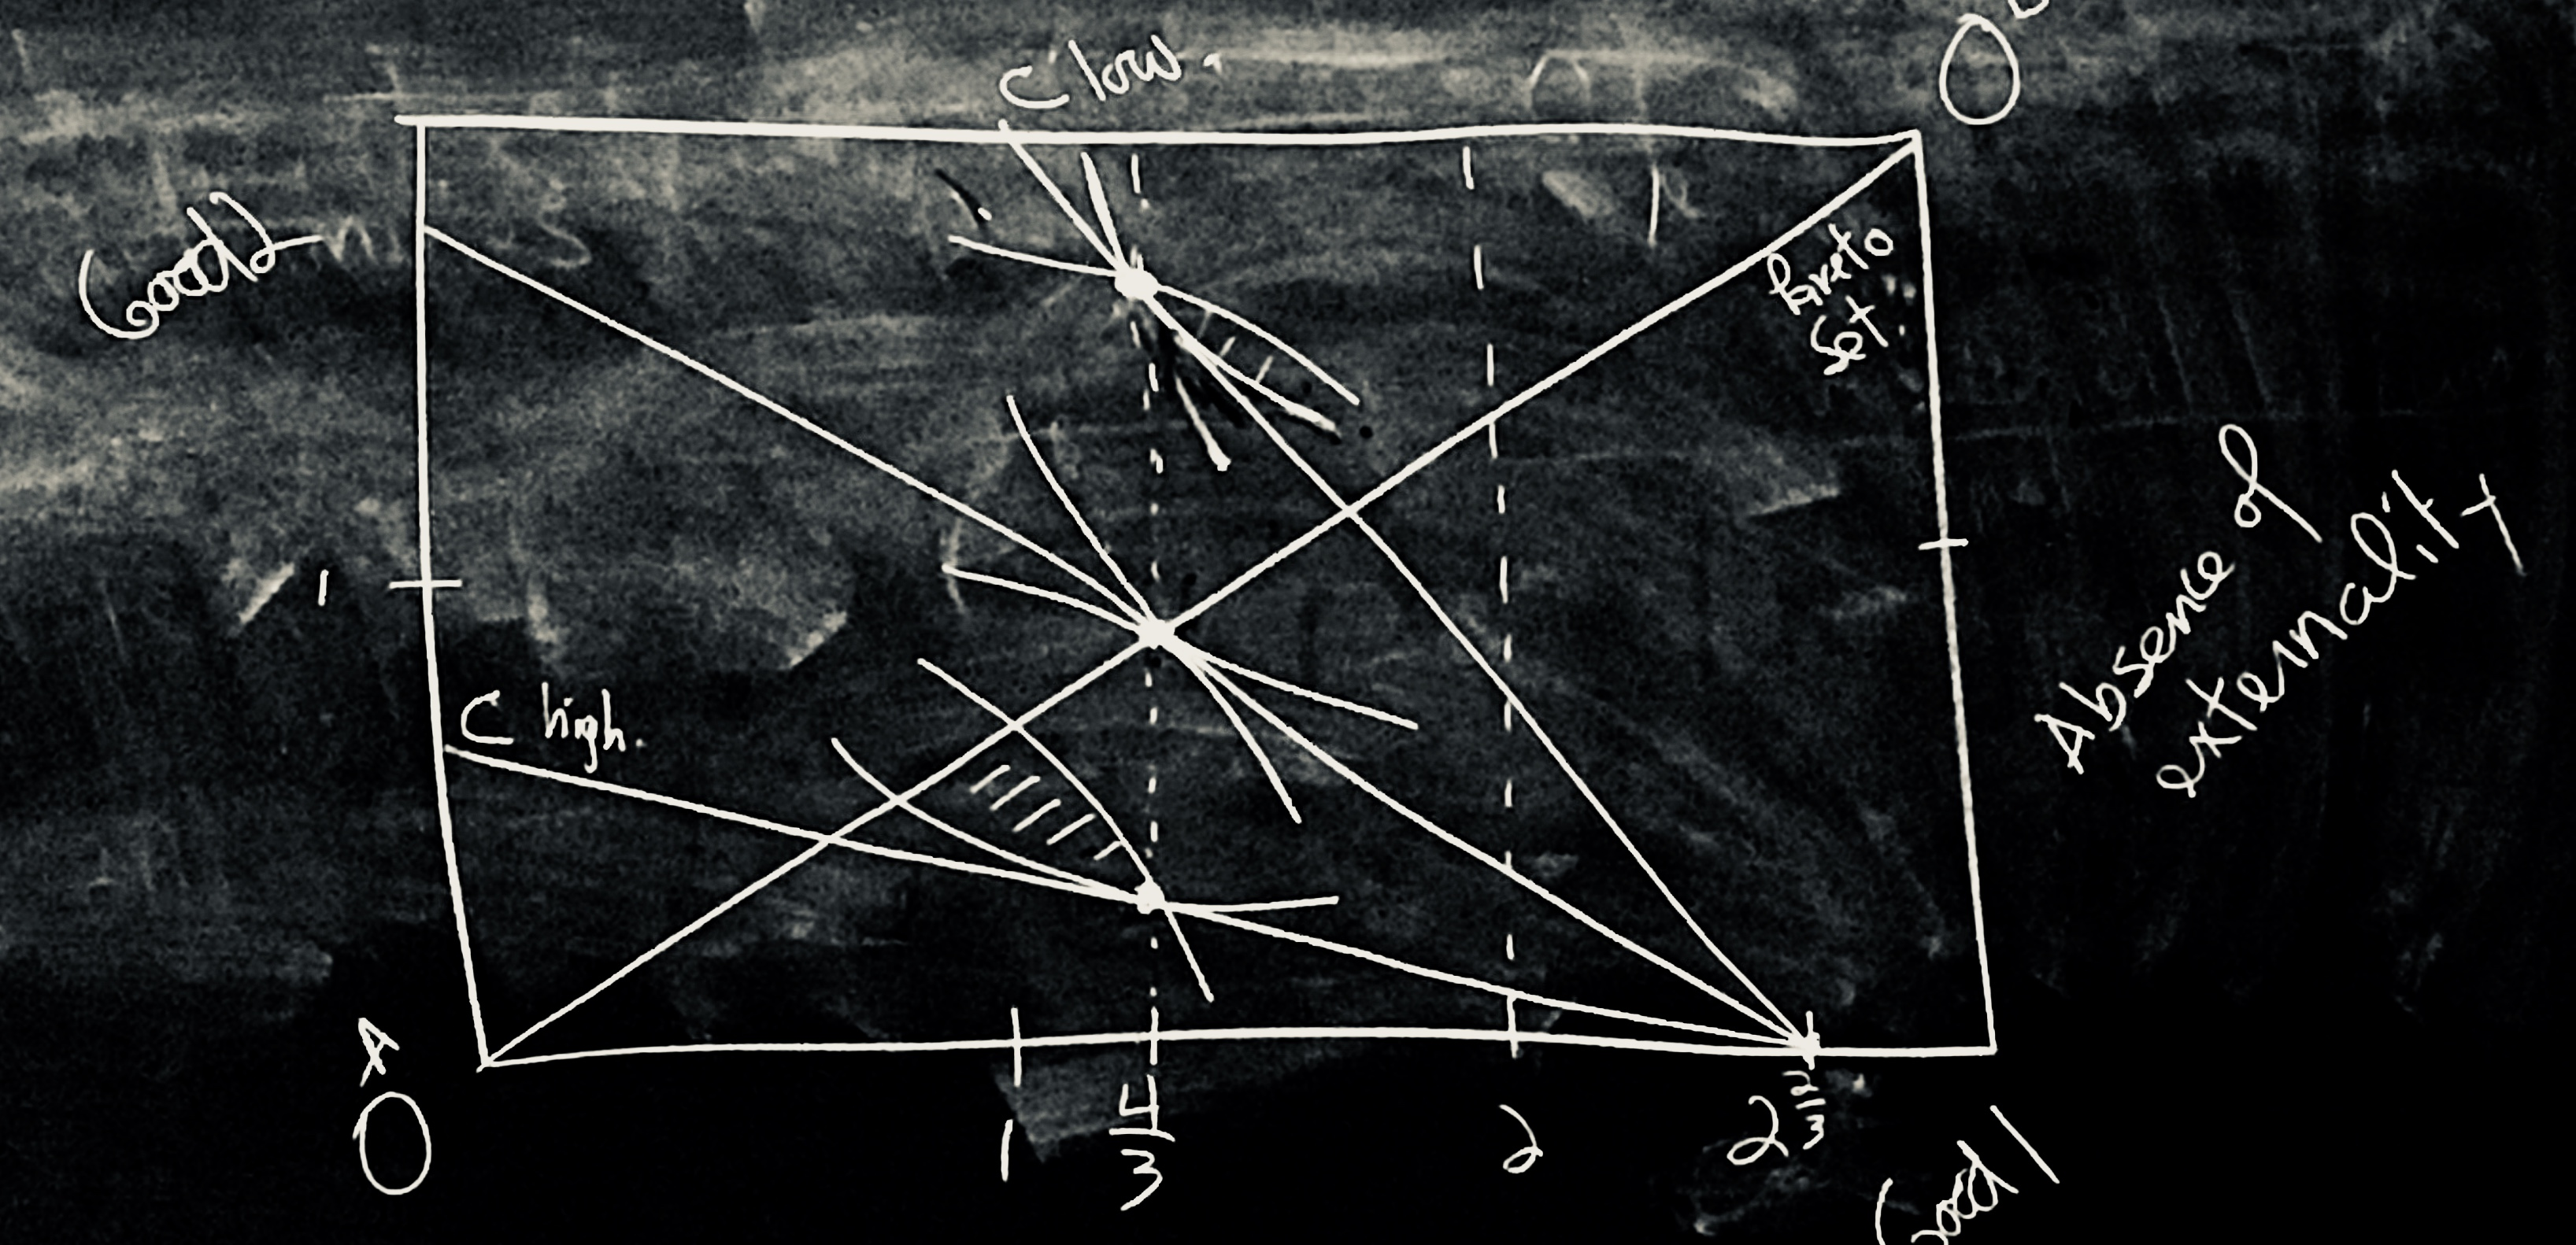
\includegraphics[scale=0.1]{32}\\
\textbf{Changing C, will pivot the budget line.}
\end{center}
\item So, government intervention can resolve inefficiencies due to externalities, but only if permit price is \(c = \frac{3}{2}\). Otherwise, resulting allocations are inefficient. 
\end{itemize}

\end{document}





